% -----------------
%  UNIVERSITY OF LIMERICK

% Template for Undergrad/Master/PhD Thesis

% Giuseppe Torre 2020
% Department of Computer Science - University of Limerick
% Also here: https://zenodo.org/record/3908239#.XvWuo_ko_6p/ 

% Based on Harish Bhanderi's PhD/MPhil template, then Uni Cambridge http://www-h.eng.cam.ac.uk/help/tpl/textprocessing/ThesisStyle/ corrected and extended in 2007 by Jakob Suckale, then MPI-CBG PhD programme  and made available through OpenWetWare.org - the free biology wiki corrected and extended   
% ------------------


%: Style file for Latex
% Most style definitions are in the external file PhDthesisPSnPDF.
% In this template package, it can be found in ./Latex/Classes/
\documentclass[oneside,12pt]{Latex/Classes/PhDthesisPSnPDF}

\usepackage{natbib}
\usepackage[style=authoryear,backend=biber]{biblatex}
\bibliography{references} % adjust this to fit your BibTex file
\usepackage{url}
\usepackage{alltt} 
\usepackage{multirow}
\usepackage{color}



\newcommand{\urlwofont}[1]
{
\urlstyle{same}\url{#1}
}

% to display Math
\usepackage{mathtools}

% to Display C++ code
\definecolor{c++red}{rgb}{0.6,0,0} % for strings
\definecolor{c++green}{rgb}{0.25,0.5,0.35} % comments
\definecolor{c++purple}{rgb}{0.5,0,0.35} % keyword
\usepackage{listings}
\lstset{language=C++}


%% Define a new 'leo' style for the package that will use a smaller font.
\makeatletter  
\def\url@leostyle{%
  \@ifundefined{selectfont}{\def\UrlFont{\sf}}{\def\UrlFont{\small\ttfamily}}}
\makeatother
%% Now actually use the newly defined style.
\urlstyle{leo}

%: Macro file for Latex
% Macros help you summarise frequently repeated Latex commands.
% Here, they are placed in an external file /Latex/Macros/MacroFile1.tex
% An macro that you may use frequently is the figuremacro (see introduction.tex)
% This file contains macros that can be called up from connected TeX files
% It helps to summarise repeated code, e.g. figure insertion (see below).

% insert a centered figure with caption and description
% parameters 1:filename, 2:title, 3:description and label
\newcommand{\figuremacro}[3]{
	\begin{figure}[htbp]
		\centering
		\includegraphics[width=1\textwidth]{#1}
		\caption[#2]{\textbf{#2} - #3}
		\label{#1}
	\end{figure}
}

% insert a centered figure with caption and description AND WIDTH
% parameters 1:filename, 2:title, 3:description and label, 4: textwidth
% textwidth 1 means as text, 0.5 means half the width of the text
\newcommand{\figuremacroW}[4]{
	\begin{figure}[htbp]
		\centering
		\includegraphics[width=#4\textwidth]{#1}
		\caption[#2]{\textbf{#2} - #3}
		\label{#1}
	\end{figure}
}

% inserts a figure with wrapped around text; only suitable for NARROW figs
% o is for outside on a double paged document; others: l, r, i(inside)
% text and figure will each be half of the document width
% note: long captions often crash with adjacent content; take care
% in general: above 2 macro produce more reliable layout
\newcommand{\figuremacroN}[3]{
	\begin{wrapfigure}{o}{0.5\textwidth}
		\centering
		\includegraphics[width=0.48\textwidth]{#1}
		\caption[#2]{{\small\textbf{#2} - #3}}
		\label{#1}
	\end{wrapfigure}
}

% predefined commands by Harish
\newcommand{\PdfPsText}[2]{
  \ifpdf
     #1
  \else
     #2
  \fi
}

\newcommand{\IncludeGraphicsH}[3]{
  \PdfPsText{\includegraphics[height=#2]{#1}}{\includegraphics[bb = #3, height=#2]{#1}}
}

\newcommand{\IncludeGraphicsW}[3]{
  \PdfPsText{\includegraphics[width=#2]{#1}}{\includegraphics[bb = #3, width=#2]{#1}}
}

\newcommand{\InsertFig}[3]{
  \begin{figure}[!htbp]
    \begin{center}
      \leavevmode
      #1
      \caption{#2}
      \label{#3}
    \end{center}
  \end{figure}
}


%%% Local Variables: 
%%% mode: latex
%%% TeX-master: "~/Documents/LaTeX/CUEDThesisPSnPDF/thesis"
%%% End: 




%: ----------------------------------------------------------------------
%:                  TITLE PAGE: name, degree,..t
% ----------------------------------------------------------------------
% below is to generate the title page with crest and author name

%if output to PDF then put the following in PDF header
\ifpdf  
    \pdfinfo { /Title  (Masters Thesis Classes)
               /Creator (TeX)
               /Producer (pdfTeX)
               /Author (Siddharth Prince sprince.ie.31@gmail.com)
               /CreationDate (D:YYYYMMDDhhmmss)  %format D:YYYYMMDDhhmmss
               /ModDate (D:YYYYMMDDhhmm)
               /Subject (Digital IHC Staining of WSIs from
H\&E Slides Using Stable Diffusion)
               /Keywords (Stable Diffusion, HER2, IHC staining,) }
    \pdfcatalog { /PageMode (/UseOutlines)
                  /OpenAction (fitbh)  }
\fi

\title{Digital IHC Staining of WSIs from
H\&E Slides Using Stable Diffusion}
% \title{Leveraging Machine Learning for Automated HER2 Scoring in Breast Cancer Pathology }



% ----------------------------------------------------------------------
% The section below defines www links/email for author and institutions
% They will appear on the title page of the PDF and can be clicked
\ifpdf
  \author{\href{mailto: sprince.ie.31@gmail.com}{Siddharth Prince}}
%  \cityofbirth{born in XYZ} % uncomment this if your university requires this
%  % If city of birth is required, also uncomment 2 sections in PhDthesisPSnPDF
%  % Just search for the "city" and you'll find them.

% here the links to the Institution you belong to
  \faculty{\href{https://www.ul.ie/scieng/schools-and-departments/department-computer-science-and-information-systems}{Department of Computer Science and Information Systems}}
  \department{\href{http://www.csis.ul.ie}{Faculty of Science and Engineering}}
  \university{\href{http://www.ul.ie}{University of Limerick}}

  % The crest is a graphics file of the logo of your research institution.
  % Place it in ./0_frontmatter/figures and specify the width
  \crest{
\includegraphics[scale=0.45]{logonew2020.jpg}}
  
% If you are not creating a PDF then use the following. The default is PDF.
%\else
 % \author{YourName}
%  \cityofbirth{born in XYZ}
 % \collegeordept{CollegeOrDept}
  %\university{University}
  %\crest{\includegraphics[width=4cm]{logo.png}}
%\fi

\renewcommand{\submittedtext}{Submitted to the University of Limerick, August 2024 in partial fulfilment of the requirements for the Degree of}
\degree{Master of Science in Artificial Intelligence \& Machine Learning}
\degreedate{}


% ----------------------------------------------------------------------
       
% turn of those nasty overfull and underfull hboxes
\hbadness=10000
\hfuzz=50pt


%: --------------------------------------------------------------
%:                  FRONT MATTER: dedications, abstract,..
% --------------------------------------------------------------

\begin{document}

%\language{english}



% sets line spacing
\renewcommand\baselinestretch{1.2}
\baselineskip=18pt plus1pt


%: ----------------------- generate cover page ------------------------

\maketitle  % command to print the title page with above variables


%: ----------------------- cover page back side ------------------------
% Your research institution may require reviewer names, etc.
% This cover back side is required by Dresden Med Fac; uncomment if needed.

\newpage


 \begin{tabbing}
1.  Supervisor: \= Dr. Ciarán Eising    \\
 \>  \= Electronic and Computer Engineering\\
 \>  \= University \emph{of} Limerick \\
 \>  \= Ireland \\
 \end{tabbing}


 \begin{tabbing}
2. Supervisor: \= Dr. James Brown \\
 \>  \= Department of Biological Sciences \\
 \>  \= University \emph{of} Limerick \\
 \>  \= Ireland \\
\end{tabbing}

\begin{tabbing}
3. Supervisor: \= Dr. Maire Lavelle \\
 \>  \= Histopathology \\
 \>  \= University Hospital Limerick \\
 \>  \= Ireland \\
\end{tabbing}


\vspace{10mm}



%: ----------------------- abstract ------------------------

% Your institution may have specific regulations if you need an abstract and where it is to be placed in the document. The default here is just after title.
%: Declaration of originality


% Thesis Abstract -----------------------------------------------------


%\begin{abstractslong}    %uncommenting this line, gives a different abstract heading
\begin{abstracts}        %this creates the heading for the abstract page

\textbf{Objective: }The purpose of this research is to explore the use of the generative AI technique, Stable Diffusion, for the creation of immunohistochemical (IHC) images 'digitally stained' from Hematoxylin and Eosin (H\&E) whole slide images(WSI) patches and classifying thereof to obtain a corresponding HER2 score. The purpose is to check if the approach provides an efficient, cost-effective, and consistent alternative to current standard practice which is known to be expensive, subjective and time-consuming for the traditional manual HER2 assessment procedure.

\textbf{Design:} We use the state-of-the-art Stable Diffusion technique implemented using a ControlNet, which is a generative AI model that allows for fine controls in the output of the generated images. 

\textbf{Results:} The fine-tuned ControlNet model generates IHC-stained image patches with the best model producing samples that have learnt a lot of the structural features of the slide. Evaluation metrics, both quantitative and qualitative are explored using comparison algorithms and the expert opinion of a pathologist.

\textbf{Conclusions:} In the present study, we show the feasibility to apply Stable Diffusion in conjunction with a ControlNet as a core technique in Digital Pathology and Stain Transfer. The use of Stable Diffusion may provide more standard and hence, reliable HER2 assessment. The study seems promising in advancing the future of AI generators in clinical digital pathology.

\textbf{Keywords:} Stable Diffusion, ControlNet, Digital Pathology, HER2 Scoring, Immunohistochemistry, Hematoxylin and Eosin, Whole Slide Images, Generative AI, Breast Cancer, Deep Learning.



\end{abstracts}
%\end{abstractlongs}


% ---------------------------------------------------------------------- 



% Thesis statement of originality -------------------------------------

% Depending on the regulations of your faculty you may need a declaration like the one below. This specific one is from the medical faculty of the university of Dresden.

\begin{declaration}        %this creates the heading for the declaration page

I herewith declare that I have produced this paper without the prohibited assistance of third parties and without making use of aids other than those specified; notions taken over directly or indirectly from other sources have been identified as such. This paper has not previously been presented in identical or similar form to any other Irish or foreign examination board.

The thesis work was conducted at the University of Limerick from May to August 2024 under the supervision of Dr. Ciarán Eising, Dr. James Brown and Dr. Máire Lavelle. 

\vspace{10mm}

Siddharth Prince  

Limerick, 2024


\end{declaration}


% ----------------------------------------------------------------------


%: ----------------------- tie in front matter ------------------------

\frontmatter

% Thesis Acknowledgements ------------------------------------------------


%\begin{acknowledgementslong} %uncommenting this line, gives a different acknowledgements heading
\begin{acknowledgements}      %this creates the heading for the acknowlegments

Your acknowledgment goes here. 
Open the acknowledgment.tex file found at: 0\_frontmatter/acknowledgment.tex

\end{acknowledgements}
%\end{acknowledgmentslong}

% ------------------------------------------------------------------------



% Thesis Dedictation ---------------------------------------------------

\begin{dedication} %this creates the heading for the dedication page

\vspace{31mm}

Your dedication  goes here. 
Open the dedication.tex file found at: 0\_frontmatter/dedication.tex

\end{dedication}

% ----------------------------------------------------------------------


%: ----------------------- contents ------------------------

\setcounter{secnumdepth}{3} % organisational level that receives a numbers
\setcounter{tocdepth}{3}    % print table of contents for level 3
\tableofcontents            % print the table of contents
% levels are: 0 - chapter, 1 - section, 2 - subsection, 3 - subsection


%: ----------------------- list of figures/tables ------------------------

\listoftables  % print list of tables
\listoffigures	% print list of figures



%: ----------------------- glossary ------------------------

% Tie in external source file for definitions: /0_frontmatter/glossary.tex
% Glossary entries can also be defined in the main text. See glossary.tex
%% this file is called up by thesis.tex
% content in this file will be fed into the main document

% Glossary entries are defined with the command \nomenclature{1}{2}
% 1 = Entry name, e.g. abbreviation; 2 = Explanation
% You can place all explanations in this separate file or declare them in the middle of the text. Either way they will be collected in the glossary.

% required to print nomenclature name to page header
\markboth{\MakeUppercase{\nomname}}{\MakeUppercase{\nomname}}


% ----------------------- contents from here ------------------------

% chemicals
\nomenclature{TRIAD}{ejfowejfopjewopfjweopjfopwejfopwjeopfjweopfjopwefjopwej} 
\nomenclature{Frame of Reference}{}
\nomenclature{IMU}{Inertial Measurement Unit}
\nomenclature{WIMU}{Wireless Inertial Measurement Unit}



 
%
%\begin{multicols}{2} % \begin{multicols}{#columns}[header text][space]
%\begin{footnotesize} % scriptsize(7) < footnotesize(8) < small (9) < normal (10)
%
%\printnomenclature[1.5cm] % [] = distance between entry and description
%\label{nom} % target name for links to glossary
%
%\end{footnotesize}
%\end{multicols}



%: --------------------------------------------------------------
%:                  MAIN DOCUMENT SECTION
% --------------------------------------------------------------

% the main text starts here with the introduction, 1st chapter,...
\mainmatter

% \renewcommand{\chaptername}{} % uncomment to print only "1" not "Chapter 1"


%: ----------------------- subdocuments ------------------------

% Parts of the thesis are included below. Rename the files as required.
% But take care that the paths match. You can also change the order of appearance by moving the include commands.


% this file is called up by thesis.tex
% content in this file will be fed into the main document

%: ----------------------- introduction file header -----------------------
\chapter{Introduction}

% the code below specifies where the figures are stored
\ifpdf
    \graphicspath{{1_introduction/figures/PNG/}{1_introduction/figures/PDF/}{1_introduction/figures/}}
\else
    \graphicspath{{1_introduction/figures/EPS/}{1_introduction/figures/}}
\fi

% ----------------------------------------------------------------------
%: ----------------------- introduction content ----------------------- 
% ----------------------------------------------------------------------

Breast cancer is one of the most prevalent cancer types among women worldwide \parencite{Sung2021GlobalCountries}, which requires proper diagnosis for planning effective treatment. As with any cancer type, early and accurate diagnosis is critical for improving patient outcomes. Given that cancer pathology is a manual and time-consuming process, machine learning (ML) techniques are making significant strides in the field of breast cancer diagnosis, offering promising avenues to complement traditional methods. A recent systematic review by \textcite{Nemade2022ATechniques} considered 162 research publications for the time period of 2015-2021 and investigated the use of machine intelligence techniques in breast cancer diagnosis. The review found that ML algorithms demonstrated promising results in tasks such as computer-aided diagnosis (CAD) using mammograms, ultrasound image analysis, and even gene expression profiling. 

One area of machine learning research that has exploded in recent years is generative AI or Foundational Models \parencite{Bommasani2021OnModels} with the introduction of Large Language Models (LLMs) such as ChatGPT \parencite{Brown2020LanguageLearners} \parencite{OpenAI2023GPT-4Report}, Gemini \parencite{GeminiTeam2023Gemini:Models}, Claude, etc., and image generation models such as Stable Diffusion \parencite{Rombach2021High-ResolutionModels}, DALL-E \parencite{Ramesh2021Zero-ShotGeneration}, Midjourney and more. Exploring new use cases for such ground breaking models is essential as they can lead to important discoveries especially in cancer research with the increasing adoption of digital pathology which opens up new avenues for the automation of diagnostic processes with increased accuracy. Whole Slide Imaging (WSI) is the complete digitization of whole tissue slides, and this has led to the application of various sophisticated computational techniques to histopathologic analysis \parencite{Aeffner2019IntroductionAssociation.} \parencite{Madabhushi2016ImageOpportunities.}.

\section{Motivation}

In this thesis, the main focus is on the Human epidermal growth factor receptor 2 (HER2). HER2 is a crucial biomarker in the pathology of breast cancer, and its over-expression is related to aggressive tumor behaviour and poor prognosis \parencite{Slamon1987HumanOncogene}. Accurate HER2 scoring is needed to determine eligibility for targeted therapies such as trastuzumab \parencite{Slamon2001UseHER2}. HER2 testing has been done traditionally through a manual HER2 score assignment from immunohistochemically (IHC) stained tissue sections. This procedure is not only time-consuming but also highly subjective, causing inter-observer variability \parencite{Wolff2013RecommendationsUpdate.}. Inevitably, the subjectivity brings forth discrepancies in diagnoses and, therefore, treatment decisions for the patients. Hence there is a need for methods that are more reliable, standardized and efficient. In the very least, a companion tool that pathologists can use to get an idea of the expected result and then verify would improve on the existing process. 

\section{Aims and Objectives} 

With the above stated problems with HER2 scoring established, this thesis investigates the application of Stable Diffusion \parencite{Rombach2021High-ResolutionModels} to generate IHC-stained WSI patches from corresponding H\&E WSI patches. Stable Diffusion has been proven to be good for high-quality, contextually accurate image generation, even better than Generative Adversarial Neural Netwoks (GANNs) that were considered to be state-of-the-art in generative models \parencite{Baranchuk2021Label-EfficientModels}. Hence Stable Diffusion is an appealing candidate for the task. The key to this is to fine-tune a pretrained Stable Diffusion model with a custom dataset containing pairs of the H\&E and IHC WSI patches. 

\vspace{5 mm}

Thus the main research questions that are aimed to be addressed in this thesis are:

\begin{enumerate}

\item Is there a visual correlation between the H\&E stain and the HER2 score of a corresponding IHC stain that may not be apparent or fully understood by human pathologists?

\item Can the current state-of-the-art generative models achieve a better result than previous work in this area where they used GANNs?

\item Can Stable Diffusion be leveraged to also output a latent representation of the image generated as a means of scoring (classification) of the generated IHC stain image?
 

\end{enumerate}

\section{Research Contribution}

As conveyed in the research questions, the initially planned scope was to not only fine-tune a pre-trained diffusion model with H\&E images as additional input to a prompt that describes the IHC score; but also to device a way for the model to output the score along with the generated IHC image while only giving the H\&E image as input. While the first part of this goal was achieved using a ControlNet \parencite{Zhang2023AddingModels} for fine-tuning the model, the latter part turned out to be beyond the scope of this thesis due to time and resource constraints. Ideas for further research for the third research question above are detailed in the future scope subsection of chapter 5. Another pertinent research area that has not been covered by this research would be to understand the morphological features of the H\&E stain that the model uses to obtain an IHC stain by using explainable AI techniques. This would help pathologists better understand the correlation and potentially also improve their own manual scoring process.

\pagebreak

\section{Thesis Outline} 

The remaining chapters of this dissertation are as follows:

\emph{Chapter Two} is an introductory discussion to Stable Diffusion and ControlNets. It also provides a review of the research that tried using GANNs for IHC stain generation which is where the main research question for this thesis was derived from. 

\emph{Chapter Three} demonstrates the implementation of the ControlNet framework which is used to fine-tune a Stable Diffusion 2.1 model.

\emph{Chapter Four} presents the results and a discussion about gauging its performance including for multiple variations of models that were trained.

\emph{Chapter Five} concludes the research and suggests possible future works that can continue the research.

\vspace{5 mm}

The Appendix A contains information about the source code used for the purposes of this dissertation. 

\vspace{5 mm}

% ----------------------------------------------------------------------



	
% this file is called up by thesis.tex
% content in this file will be fed into the main document

%: ----------------------- name of chapter  -------------------------

\chapter{Literature Survey} % top level followed by section, subsection

%: ----------------------- paths to graphics ------------------------

% change according to folder and file names
\ifpdf
    \graphicspath{{2_chapter2/figures/PNG/}{2_chapter2/figures/PDF/}{2_chapter2/figures/}}
\else
    \graphicspath{{2_chapter2/figures/EPS/}{2_chapter2/figures/}}
\fi

%: ----------------------- contents from here ------------------------

Latex will automatically renumber sections! Also it creates list of figures, list of tables and references! Nice job!


This document is formatted according to the University of Limerick specification for the submission of a Master or PhD dissertation.
Double-page printing is already in the code!
If you want to change things  you need to modify the `PhDthesisPSnPDF.cls' file found in Latex/Classes 




\section{Font}

Normal font \textbf{Bold Font} \emph{italics}.  List of \textcolor{blue}{colours} \textcolor{red}{for} \textcolor{ForestGreen}{font} can be found at: \url{http://en.wikibooks.org/wiki/LaTeX/Colors}

\subsection{Special characters}

Special characters such as \& and \% need to be treated in a special way. Check the full list of special characters here: \url{http://en.wikibooks.org/wiki/LaTeX/Special_Characters}
\subsubsection{Subsubsection Title}

\subsection{Wiki page}

You can learn more about Latex by clicking \href{http://en.wikibooks.org/wiki/LaTeX}{here}.


\section{Another Section}

\subsection{Another Subsection}

\subsubsection{Another Subsubsection Title}




% ---------------------------------------------------------------------------
%: ----------------------- end of thesis sub-document ------------------------
% ---------------------------------------------------------------------------


% this file is called up by thesis.tex
% content in this file will be fed into the main document

\chapter{Dataset} % top level followed by section, subsection

\ifpdf
    \graphicspath{{3_chapter3/figures/PNG/}{3_chapter3/figures/PDF/}{3_chapter3/figures/}}
\else
    \graphicspath{{3_chapter3/figures/EPS/}{3_chapter3/figures/}}
\fi

% ----------------------- contents from here ------------------------




\section{Insert a Figure}
 We refer to a figure in the text like this:  (Figure \ref{image02}).
 
 \figuremacroW{image02}{Title of Figure}{Description. [Source: (\Citealt{mydownloadedimage})]}{0.7} 
 


\section{Creating a list}

\begin{itemize} \itemsep1pt \parskip0pt \parsep0pt
\item \textbf{(2000)} item 1. 
\item \textbf{(2004)} item 2. 
\item \textbf{(2010)} item 3. 
\item \textbf{(2013)} item 4. 
\end{itemize}


\subsection{Creating a Table}

\begin{table}[htpp]
\caption{Table Title}
\begin{center}
\begin{tabular}{| p{3cm} | c | c | c |}
\hline 
 & Resolution & Min & Max \\ \hline 
Gyroscope & 4.5mV / {$^{\circ}$}/s & 0.27 $^{\circ}$/s & 406 $^{\circ}$/s \\ \hline
Accelerometer & 600mV /g &  0.002g & 2g \\ \hline
Magnetometer & 385mV/ gauss & 0.317 gauss & 6 gauss \\ \hline
\end{tabular}
\end{center}
\label{Sensors' Resolution}
\end{table}%


% here is how to do a page break
\pagebreak
%done

\section{Quote}
 An in-text quote is declared in the following way:

\begin{quote}

Recycling is the way forward! Recycling is the way forward! Recycling is the way forward! Recycling is the way forward! Recycling is the way forward! Recycling is the way forward! Recycling is the way forward! Recycling is the way forward! Recycling is the way forward! Recycling is the way forward! Recycling is the way forward! Recycling is the way forward! Recycling is the way forward! Recycling is the way forward! Recycling is the way forward! Recycling is the way forward! Recycling is the way forward! Recycling is the way forward! Recycling is the way forward!    (CommonSense, p. 0) 

 \end{quote}

Another way of doing it is:
\begin{quote}
{
\centering
\emph{There are in our existence spots of time, \\
That with distinct pre-eminence retain \\
A renovating virtue, whence-depressed \\
By false opinion and contentious thought, \\
Or aught of heavier or more deadly weight, \\
In trivial occupations, and the round \\
Of ordinary intercourse-our minds \\ 
Are nourished and invisibly repaired; \\ 
A virtue, by which pleasure is enhanced, \\ 
That penetrates, enables us to mount, \\ 
When high, more high, and lifts us up when fallen. \\ 
}

(\Citealt[verses 208-218]{poem})

}


\end{quote}








% ---------------------------------------------------------------------------
% ----------------------- end of thesis sub-document ------------------------
% ---------------------------------------------------------------------------			
% this file is called up by thesis.tex
% content in this file will be fed into the main document

\chapter{Research Methodology} % top level followed by section, subsection


% ----------------------- paths to graphics ------------------------

% change according to folder and file names
\ifpdf
    \graphicspath{{4_ResearchMethodology/figures/PNG/}{4_ResearchMethodology/figures/PDF/}{4_ResearchMethodology/figures/}}
\else
    \graphicspath{{4_ResearchMethodology/figures/EPS/}{4_ResearchMethodology/figures/}}
\fi


% ----------------------- contents from here ------------------------

\section{Data Preparation}

This is achieved by methods of projection transformation and elastix registration \parencite{Klein2010Elastix:Registration}  with the former resulting in a rough overlap between the two image types and subsequently the latter performing a "regional fine-grained non-rigid registration" \parencite[p. 5]{Liu2022BCI:Pix2pix}. 

- No real data pre-processing/manipulation done - limit test of how well SD will work

\subsection{Data Distribution}

\section{ControlNet Implementation}

\subsection{System Specifications}

\subsection{Training}

\section{Evaluation}



% ---------------------------------------------------------------------------
% ----------------------- end of thesis sub-document ------------------------
% ---------------------------------------------------------------------------
% this file is called up by thesis.tex
% content in this file will be fed into the main document



%: ----------------------- name of chapter  -------------------------
\chapter{Results} % top level followed by section, subsection

\ifpdf
    \graphicspath{{5_Results/figures/PNG/}{5_Results/figures/PDF/}{5_Results/figures/}}
\else
    \graphicspath{{5_Results/figures/EPS/}{5_Results/figures/}}
\fi

This chapter consists of discussions about the various results and performance metrics gathered over the course of training and testing the models. First, further training metrics are discussed and then the results from testing are considered.

\section{Training Loss}

\subsection{Model variation 1: SD Locked}

This was the best performing model out of the two with stark differences in the quality of generated images being observed even at the training phase. The Figures \ref{fig:mod1-train-loss-epoch} and \ref{fig:mod1-train-loss-epoch-smooth} represent the same loss with loss value plotted against number of epochs. From the first graph we can see that the loss has been very erratic and it unable to get to a convergence point. In fact, at around 20k steps ($\approx 20  epochs$), the epoch loss has managed to reach the lowest loss of 0.1763 while the last epoch i.e., 50 ended the training with the second lowest of 0.1778. The immediate realisation is that learning rate would need to be lowered.
\begin{figure}[h]
    \centering
    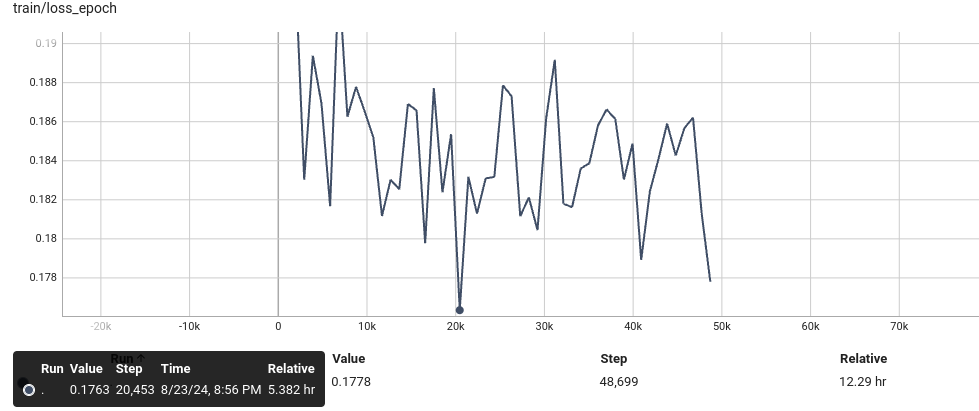
\includegraphics[width=1\linewidth]{5_Results/figures/var1-train-epoch-loss.png}
    \caption{Model 1: Train loss/epoch}
    \label{fig:mod1-train-loss-epoch}
\end{figure}
But when the smoothed curve is observed, there is an overall down slope to the learning which suggests that the training is in general moving in a positive direction but perhaps it would yield better results if the number of epochs were to be increased and training continued for a longer period of time. In fact, 50 epochs is not a high number at all when most such training projects train for epochs in the range of thousands. There is also an interesting note observed by the author \parencite[Figure 4, p. 5]{Zhang2023AddingModels} where the phenomenon of sudden convergence is observed after enough training steps. It should also be noted that ControlNets are mainly used with adding image masks such as depth, edge, segmentation maps as their control input for training which would contain way lesser spatial and structural data and more rigidity to the outcomes. With our use case being two different staining domains, these variations in performance is to be expected. 
\begin{figure}[h]
    \centering
    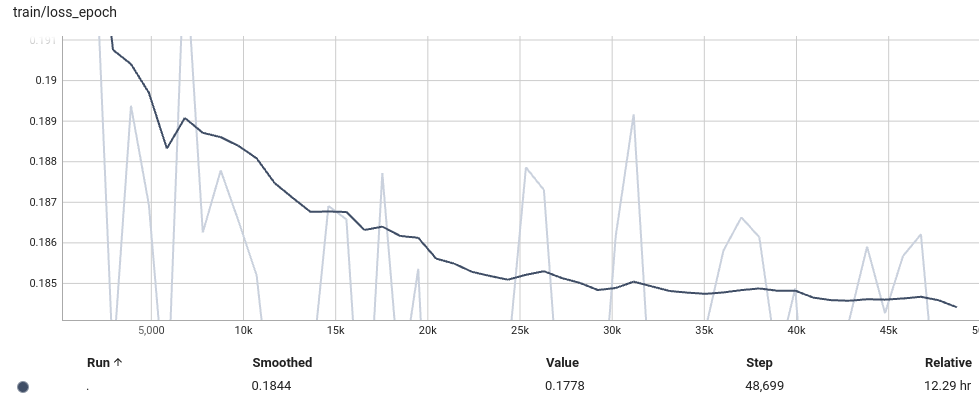
\includegraphics[width=1\linewidth]{5_Results/figures/model-1-train-loss-epoch-smooth.png}
    \caption{Model 1: Train loss/epoch with smoothing=0.9}
    \label{fig:mod1-train-loss-epoch-smooth}
\end{figure}

The four Figures \ref{fig:train-log-source-e20-s900}, \ref{fig:train-log-target-e20-s900}, \ref{fig:train-log-sample-e20-s900} and \ref{fig:train-log-prompt-e20-s900} is a training render sample that corresponds to the $900^{th}$ step in epoch 20 of training which is where the least loss was observed. This too has good structural and intensity mapping in the generated images. The colouring on the membranes of the cells and the patterns formed are very much comparable when performing a the simple eye test.
\begin{figure}[h]
    \centering
    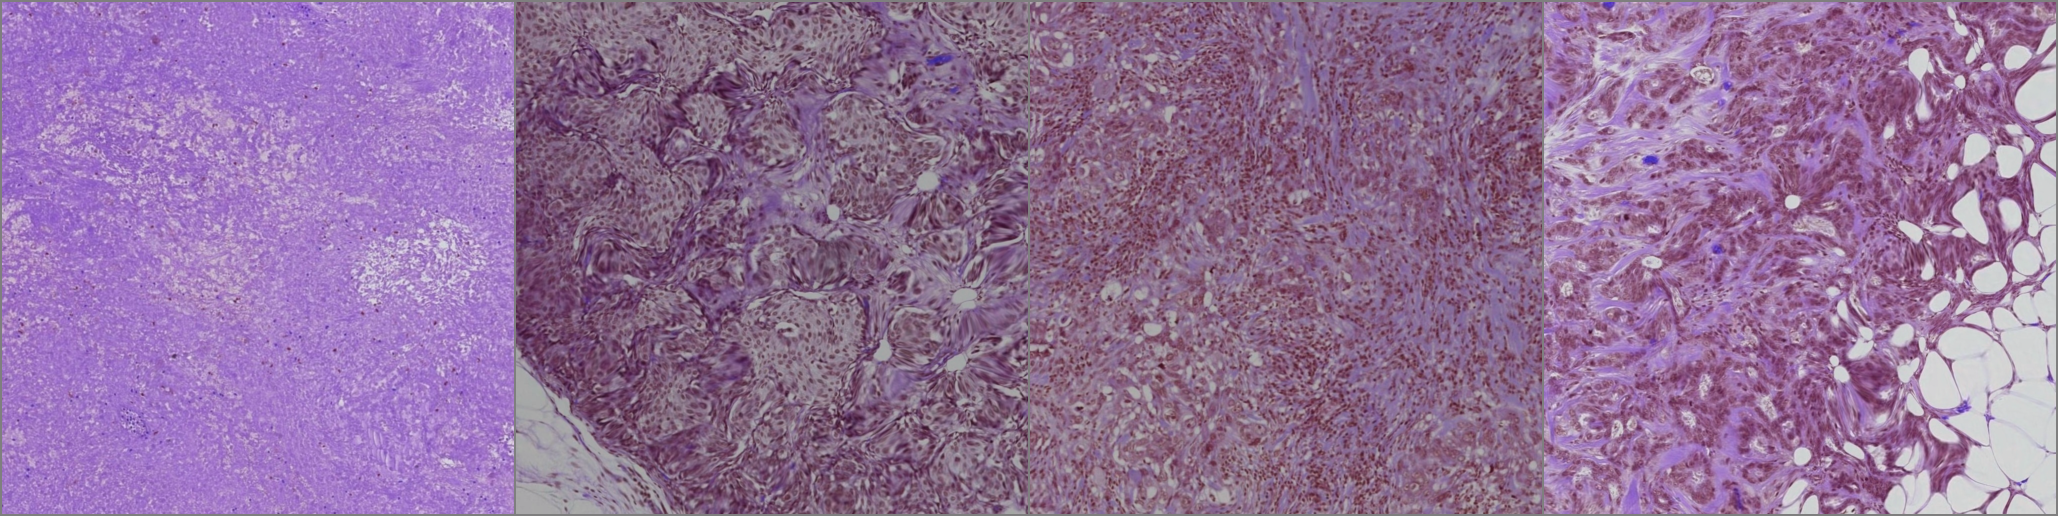
\includegraphics[width=1\linewidth]{5_Results/figures/control_gs-020380_e-000020_b-000900.png}
    \caption[Input H\&E images for train log at e=20, steps=900]{H\&E Stain - Input}
    \label{fig:train-log-source-e20-s900}
\end{figure}
\begin{figure}[h]
    \centering
    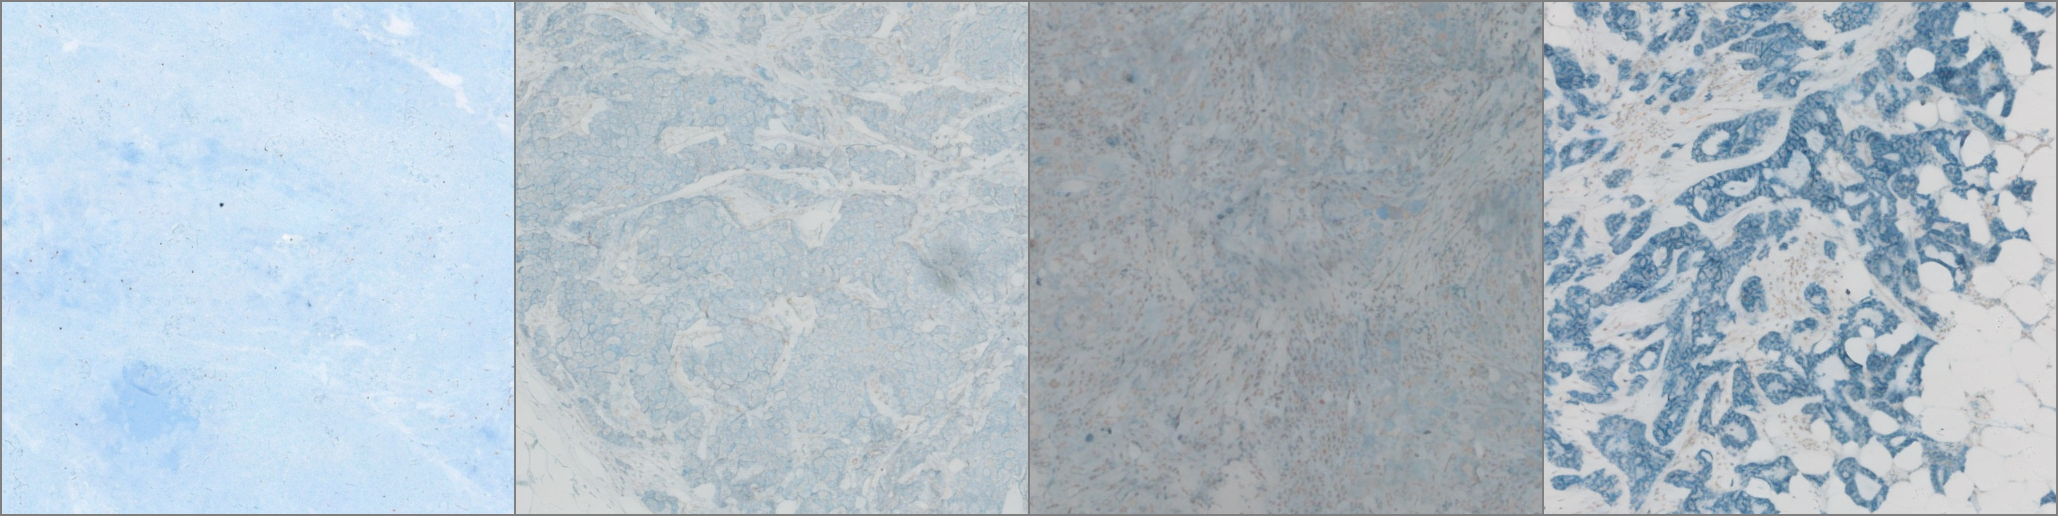
\includegraphics[width=1\linewidth]{5_Results/figures/reconstruction_gs-020380_e-000020_b-000900.png}
    \caption[Target IHC images for train log at e=20, steps=900]{IHC Stain - Ground Truth}
    \label{fig:train-log-target-e20-s900}
\end{figure}
\begin{figure}[h]
    \centering
    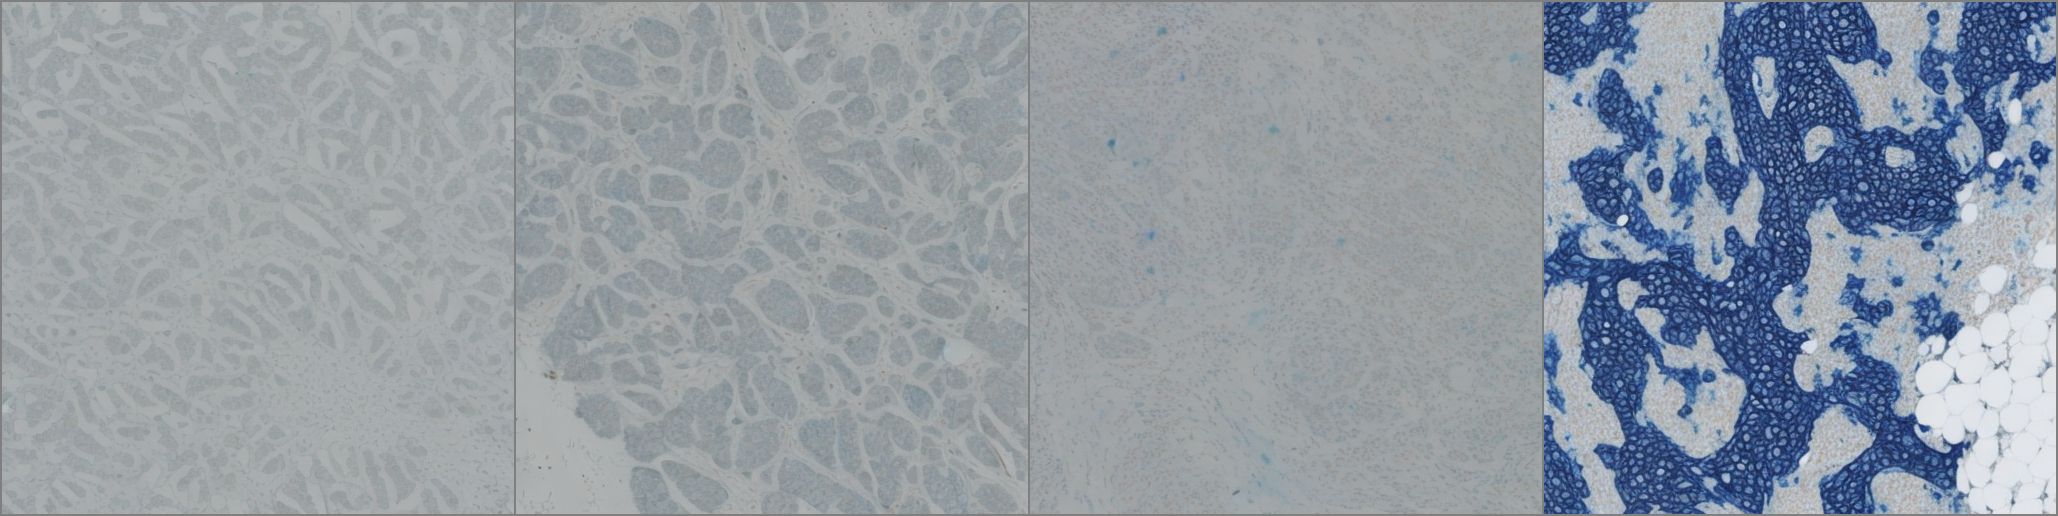
\includegraphics[width=1\linewidth]{5_Results/figures/samples_cfg_scale_9.00_gs-020380_e-000020_b-000900.png}
    \caption[Generated IHC images for train log at e=20, steps=900]{IHC Stain - Generated}
    \label{fig:train-log-sample-e20-s900}
\end{figure}
\begin{figure}[h]
    \centering
    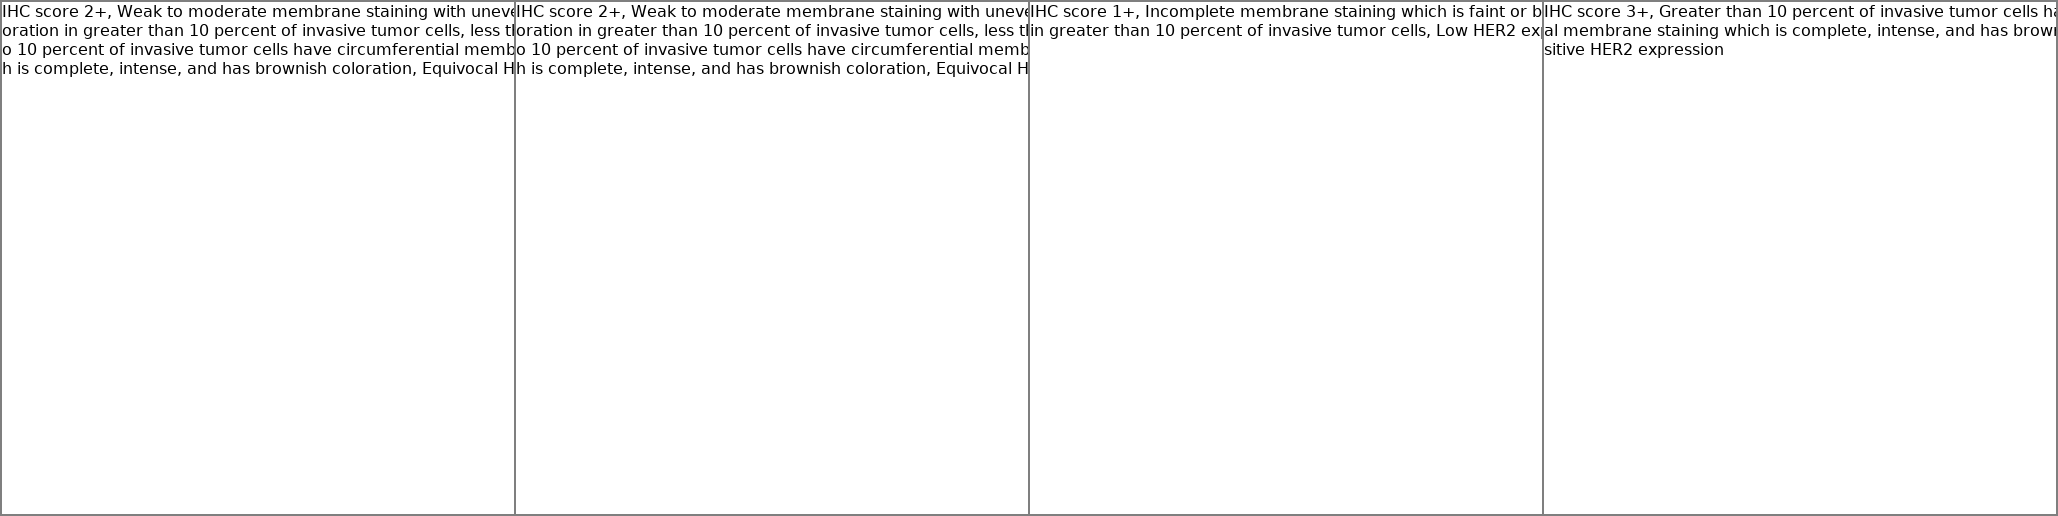
\includegraphics[width=1\linewidth]{5_Results/figures/conditioning_gs-020380_e-000020_b-000900.png}
    \caption[Input prompts for train log at e=20, steps=900]{IHC Score + Prompt. IHC scores from left to right are 2+. 2+. 1+ and 3+}
    \label{fig:train-log-prompt-e20-s900}
\end{figure}

\subsection{Model variation 1: SD Unlocked}

From the loss metrics of Figures \ref{fig:mod2-train-loss-epoch} and \ref{fig:mod2-train-loss-epoch-smooth}, there is a lot more variability here between epochs. The smoothed graph also suggests a plateaued trend line. But, from the loss curve, we can see that the penultimate epoch of 49 achieved a loss of 0.1756 which is slightly lower than the least value from model 1. This seems to suggest that training the SD layers along with the copy has the potential for better fitting with the objective but the number of epochs might again be too low to make any definitive conclusion.
\begin{figure}[h]
    \centering
    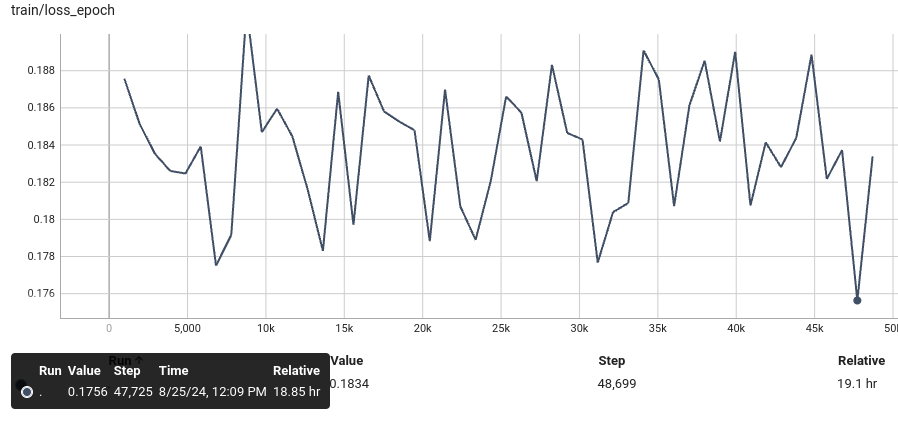
\includegraphics[width=1\linewidth]{5_Results/figures/sd2-train-loss-epoch.png}
    \caption{Model 2: Train loss/epoch}
    \label{fig:mod2-train-loss-epoch}
\end{figure}

\begin{figure}[h]
    \centering
    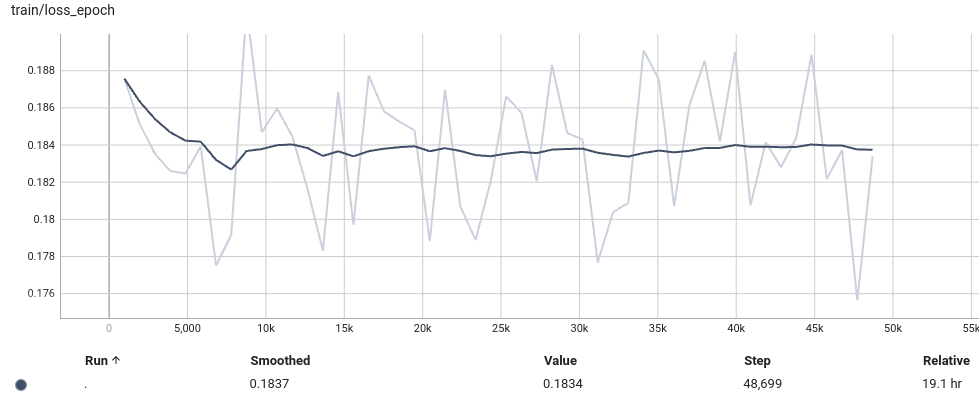
\includegraphics[width=1\linewidth]{5_Results/figures/model-2-train-epoch-loss-smooth.png}
    \caption{Model 2: Train loss/epoch with smoothing=0.9}
    \label{fig:mod2-train-loss-epoch-smooth}
\end{figure}

\section{Objective Evaluation}

As discussed in section 3.3.2, objective evaluation of the test results is not ideal to gauge the effectiveness of the trained model. The results are tabulated in Table \ref{tab:obj-results}.

\begin{table}[H]
\begin{center}
\begin{tabular}{|>{\raggedright\arraybackslash}p{0.3\linewidth}|>{\raggedright\arraybackslash}p{0.35\linewidth}|>{\raggedright\arraybackslash}p{0.35\linewidth}|}
\hline 
\textbf{Model}& \textbf{PSNR(dB)}& \textbf{SSIM}\\ \hline 
CycleGAN& 16.203& 0.373\\ \hline
pix2pix(unet generator)& 18.654& 0.419\\ \hline
Pyramid pix2pix& \textbf{21.160}& \textbf{0.477}\\ \hline
SD Locked (with prompt)& 14.54& 0.3808\\ \hline
SD Locked (without prompt)& 11.86& 0.3084\\ \hline
\end{tabular}
\caption[PSNR and SSIM metrics for the models discussed]{PSNR and SSIM metrics for the models discussed. Note that the CycleGAN and two pix2pix implementation metrics have been taken from \textcite{Liu2022BCI:Pix2pix}[Table 1, p. 7]}\label{tab:obj-results}
\end{center}
\end{table}

From these metrics, the Pyramid pix2pix model is still the one to beat by a long shot compared to our models. The only gain than any other model is in the SSIM category against CycleGAN which is already relatively obsolute for this field. Also, as expected, the model tested with the prompt is the better performing model with a 0.08 point lead compared to the test without prompts ad isn't too bad compared to pix2pix(unet). This gives hope that considering for how little time it was trained, there and the loss trend, there is alot of growth for improvement with just more training and experimentation with hyper-parameters like learning rate.

\section{Subjective Validation}

\begin{figure}[h]
    \centering
    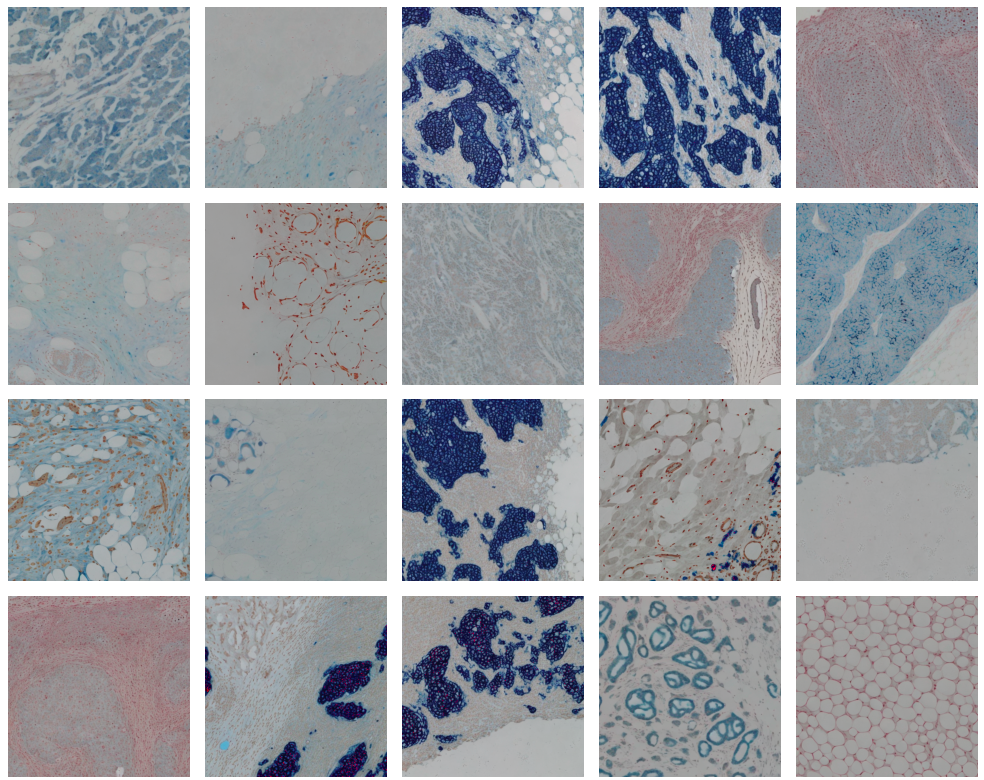
\includegraphics[width=1\linewidth]{5_Results/figures/subjective-eval-samples.png}
    \caption{A grid of 20 randomly selected generated IHC image patches for subjective validation}
    \label{fig:sub-eval-grid}
\end{figure}

For the subjective validation of manual scoring of 20 random generated IHC images the accuracy turned out to be on par with the highest accuracy obtained by two independent pathologists in the case of \textcite{Liu2022BCI:Pix2pix}[Table 5, p. 8] which \textbf{40\%}. Now, this is not an extensive sample size and in the paper they selected 40 images instead of 20. But again, as we've seen in previous examples, there is a lot of potential.

\begin{figure}[h]
    \centering
    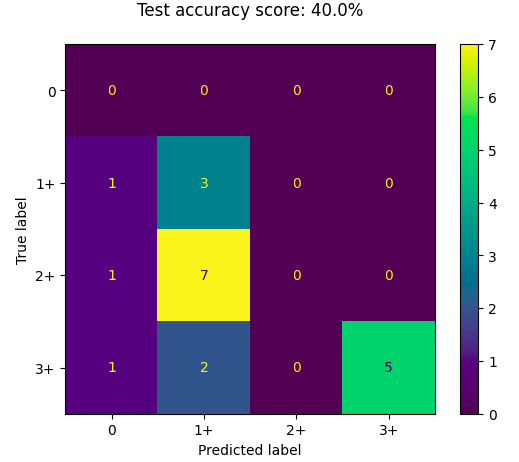
\includegraphics[width=1\linewidth]{5_Results/figures/subj-eval-confusion-matrix.png}
    \caption{Confusion matrix report of subjective validation resilts}
    \label{fig:conf-mat}
\end{figure}

Figure \ref{fig:conf-mat} shows the various accuracies across the four classes with 3+ performing the best understandably because these images have the most distinguishable morphological features standing out from the IHC stain. 2+ had a zero percent accuracy with it being mistaken for the 1+ class over 7 times by the model. There are also no successful class 0 predictions and the lack of candidates in the sample size again points out the data imbalance issue with the dataset.

\section{Key Limitations}

The biggest limitation with the research performed in this thesis is that the trained model is purely generative and does not have the capabilities to act as a classifier which is what we would want and was part of the original research goals. It just ended out to be out of the scope for this master's thesis on account of time and resource constraints. Thus in its current state, the trained model does not pose any real world application and is best to be considered a proof-of-concept of Stable Diffusion's capability in conjunction with ControlNet. 

The second key limitation in the methodology of this research is the lack of variable experimentation with different hyper-parameters which would have potentially yielded better results.

% ---------------------------------------------------------------------------
%: ----------------------- end of thesis sub-document ------------------------
% ---------------------------------------------------------------------------

	
% this file is called up by thesis.tex
% content in this file will be fed into the main document

\chapter{Conclusion and Future Directions } % top level followed by section, subsection


% ----------------------- paths to graphics ------------------------

% change according to folder and file names
\ifpdf
    \graphicspath{{6_conclusions/figures/PNG/}{6_conclusions/figures/PDF/}{6_conclusions/figures/}}
\else
    \graphicspath{{6_conclusions/figures/EPS/}{6_conclusions/figures/}}
\fi


% ----------------------- contents from here ------------------------

\section{Future Work}

With future directions in which research can be taken, probably the most obvious one would be to simply continue training the model for significantly more number of epochs. The second intuitive choice would be to now train the fine-tuned SD locked model without prompt input so that it could potentially learn to distinguish between classes with just the H\&E image inputs. A good idea to gradually help the model learn these mappings would be to perform gradual masking of the text prompts over time until no prompts are used. This could theoretically help the model converge faster than if the prompts were just disabled altogether. 

Other more experimental approaches would be to try different combinations of the ideas proposed by latest research in this field such as adding discriminator blocks from the GAN architecture to the Stable Diffusion pipeline \parencite{Wang2022Diffusion-GAN:Diffusion}, using better optimised loss functions for training such as the Pyramid pix2pix \parencite{Liu2022BCI:Pix2pix}
or the method proposed by \textcite{Ma2024DSFF-GAN:Cancer}, DSFF-GAN.

Some good data preprocessing that can be done to improve results would be to normalise image colours before training the model. Having a lot of variability in the image properties such as image contrast and colour intensity will lead to lesser accurate learning as was the case in this thesis. Also, always finding varied data sources will improve the robustness of learning and not make it overfit on just one dataset. However, this has never been a very accessible task when it comes to medical data.

A final idea to take this project forward with could be to explore reinforcement learning techniques with the ControlNet architecture for a different approach to handling loss during training.

\section{Conclusions}

Overall this body of research aimed to explore the application and efficacy of new and cutting-edge generative model. Of the three research questions posed, the first two have been explored where the results showed a definite degree of morphological parallels between the H\&E and HER2 IHC patches. For the second research question of training this model to perform better than the current state-of-the-art models, it did not achieve that but given that qualitative analysis, though the result comparison not perfect, being on par with the research this thesis was based up on is a definite positive. The final research question of training the SD model to act as a classifier while also generating IHC images was not able to be realised and is the biggest limitation. The latest literature was reviewed and many decisions in implementation was done based off this. The results were analysed and discussed in a way that would make sense for the nature of the generative image research and followed evaluation metrics followed by other research in this field.

The stain transfer area of research though niche, is promising with many cutting-edge generative techniques being researched to improve the quality-of-life for pathologists and cancer patients alike. Discovering and inventing better technology to fight and contribute to the fight against cancer is always a noble pursuit. Demonstrating the capabilities of the model in this thesis with less training cycles proves that this pursuit is worth pursuing. 


% ---------------------------------------------------------------------------
% ----------------------- end of thesis sub-document ------------------------
% --------------------------------------------------------------------------- 
\include{8_References/references}

% for reference list see line 361
% description of lab methods




% --------------------------------------------------------------
%:                  BACK MATTER: appendices, refs,..
% --------------------------------------------------------------

% the back matter: appendix and references close the thesis



%: ----------------------- bibliography ------------------------

% \begin{small} % tiny(5) < scriptsize(7) < footnotesize(8) < small (9)

\renewcommand{\bibname}{References} % changes the header; default: Bibliography
\printbibliography
% \end{small}

%\end{multicols}

% --------------------------------------------------------------
% Various bibliography styles exit. Replace above style as desired.

% in-text refs: (1) (1; 2)
% ref list: alphabetical; author(s) in small caps; initials last name; page(s)
%\bibliographystyle{Latex/Classes/PhDbiblio-case} % title forced lower case
%\bibliographystyle{Latex/Classes/PhDbiblio-bold} % title as in bibtex but bold
%\bibliographystyle{Latex/Classes/PhDbiblio-url} % bold + www link if provided

%\bibliographystyle{Latex/Classes/jmb} % calls style file jmb.bst
% in-text refs: author (year) without brackets
% ref list: alphabetical; author(s) in normal font; last name, initials; page(s)

%\bibliographystyle{plainnat} % calls style file plainnat.bst
% in-text refs: author (year) without brackets
% (this works with package natbib)


% -------------------------------------------------------------

\end{document}
